\documentclass{gost}

%-------------------------------------------------------------------------------
%
% ПЕРЕМЕННЫЕ
%
%-------------------------------------------------------------------------------

\newcommand{\universityFullName}{Федеральное государственное бюджетное
образовательное учреждение высшего образования Саратовский Государственный
Технический Университет имени Гагарина Ю.А.}
\newcommand{\universityShortName}{СГТУ им. Гагарина Ю.А.}
\newcommand{\department}{Прикладные информационные технологии}
\newcommand{\nirName}{Лабораторная работа по основам работы с разделами жесткого
диска и файловой системой в ОС Unix}
\newcommand{\nirType}{заключительный}
\newcommand{\subject}{Программные и аппаратные технологии умного города}

%-------------------------------------------------------------------------------
%
% ДОКУМЕНТ
%
%-------------------------------------------------------------------------------

\begin{document}
	\gostTitlePage

	\section{Изменение размера swap}
		\begin{figure}[H]
			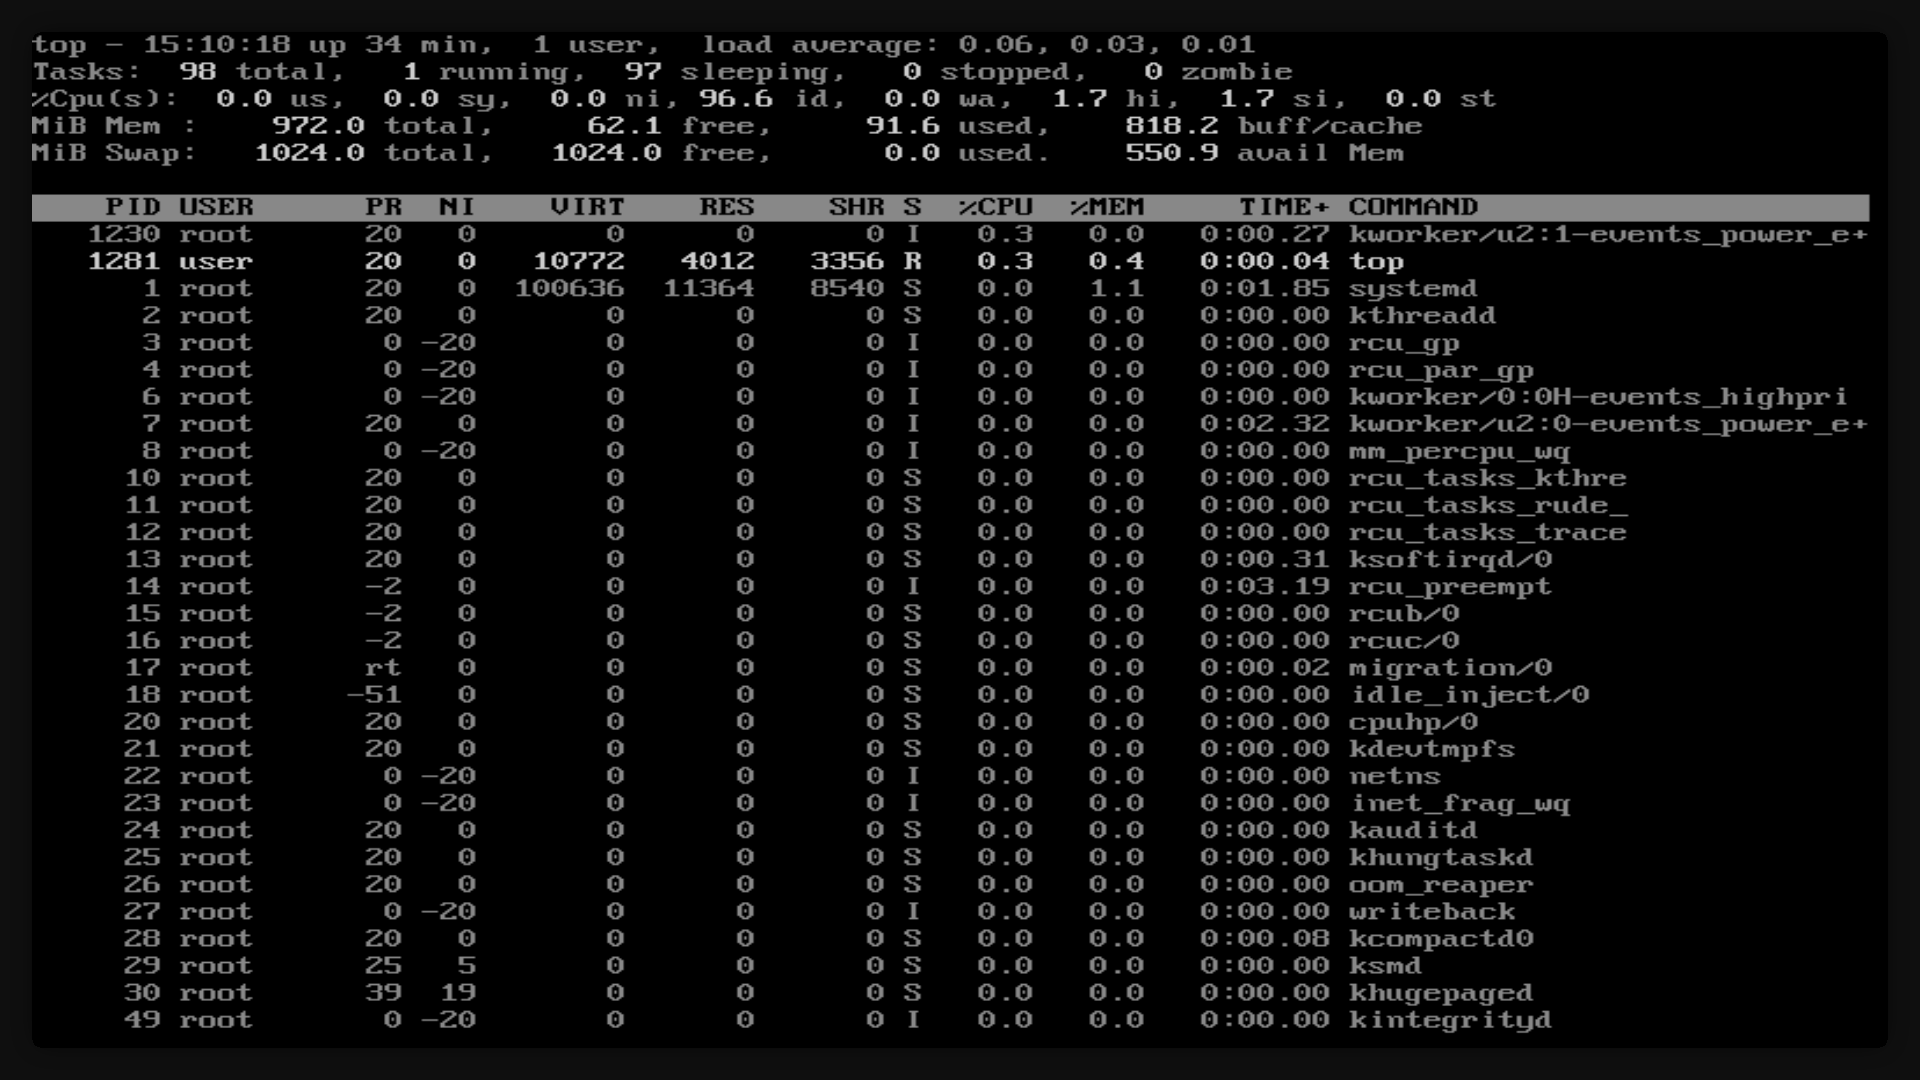
\includegraphics[width=\textwidth,clip=true]{img/1.png}
			\caption{Проверяем объем файла подкачки, который на представленном
			скриншоте равен нулю}
		\end{figure}

		\begin{figure}[H]
			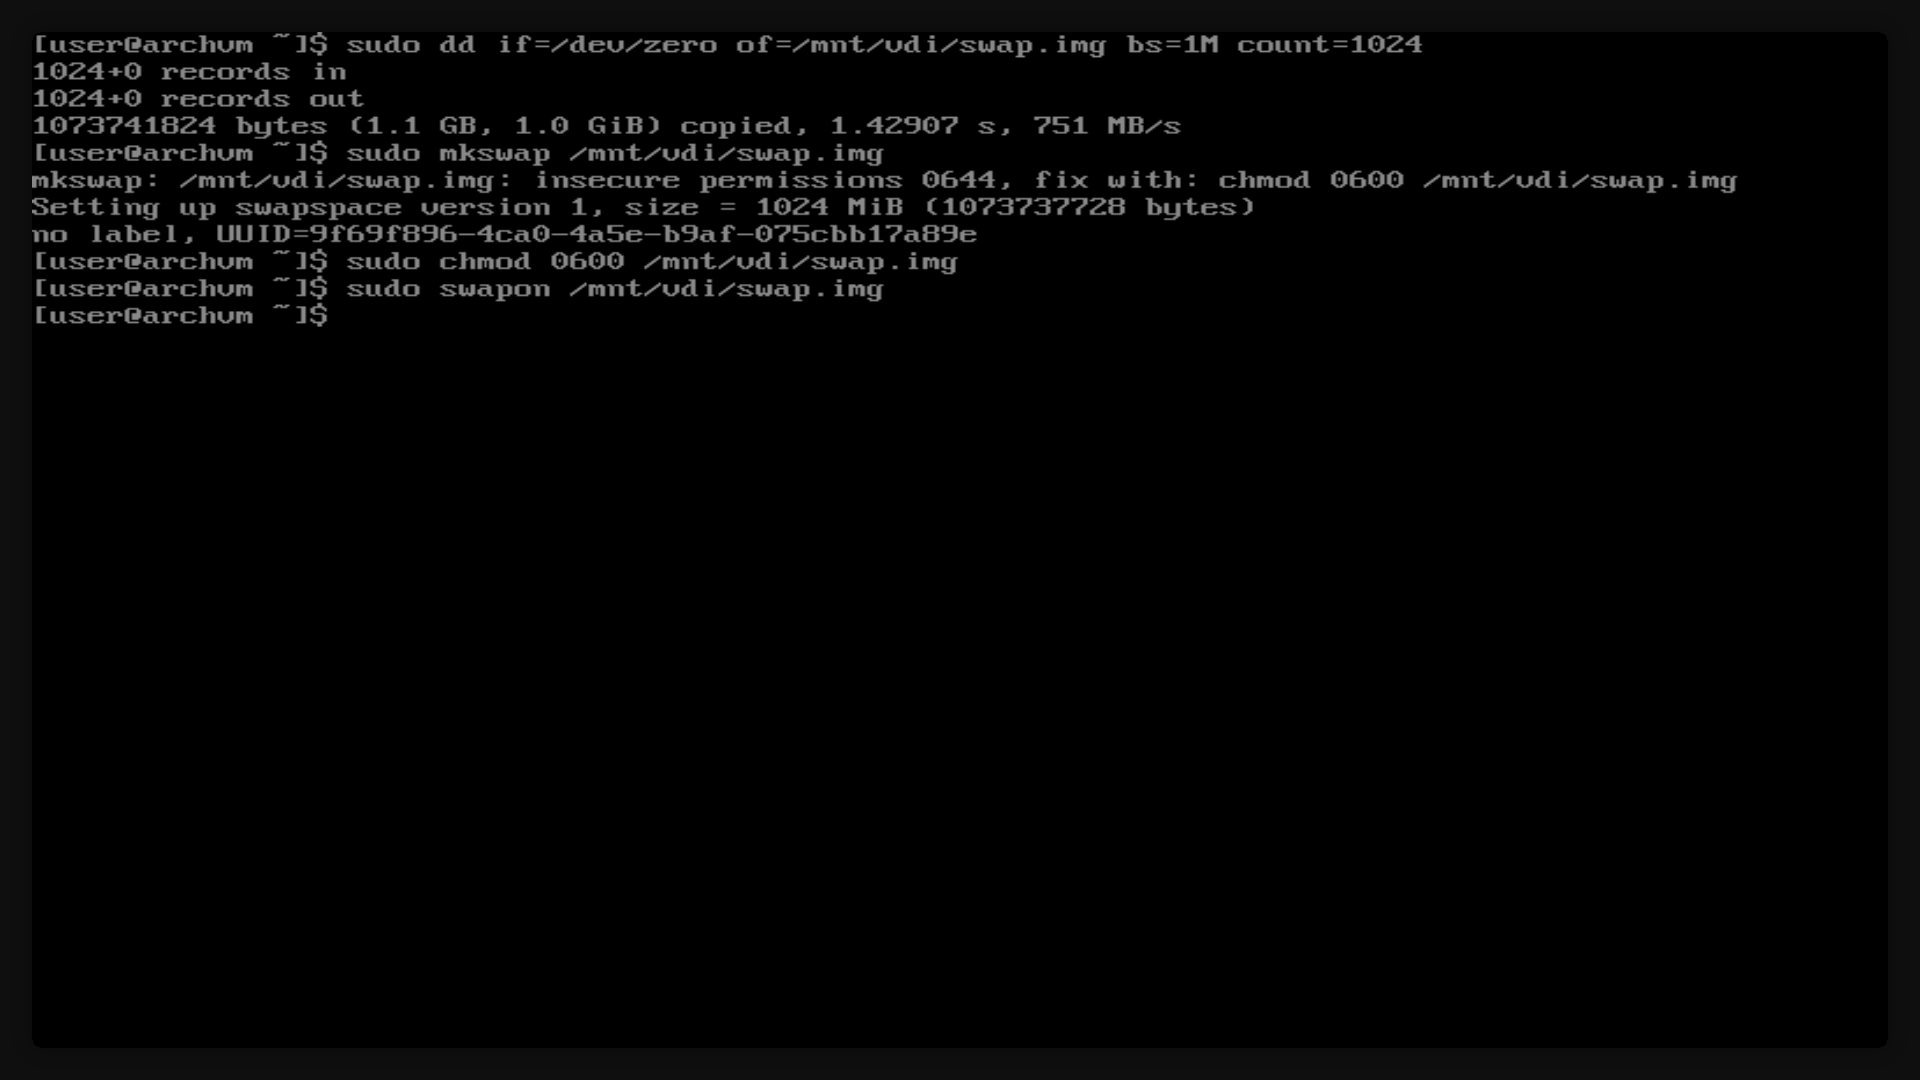
\includegraphics[width=\textwidth,clip=true]{img/2.png}
			\caption{Создаем файл размером 1024 MиБ и подключаем его как swap-раздел}
		\end{figure}

		\begin{figure}[H]
			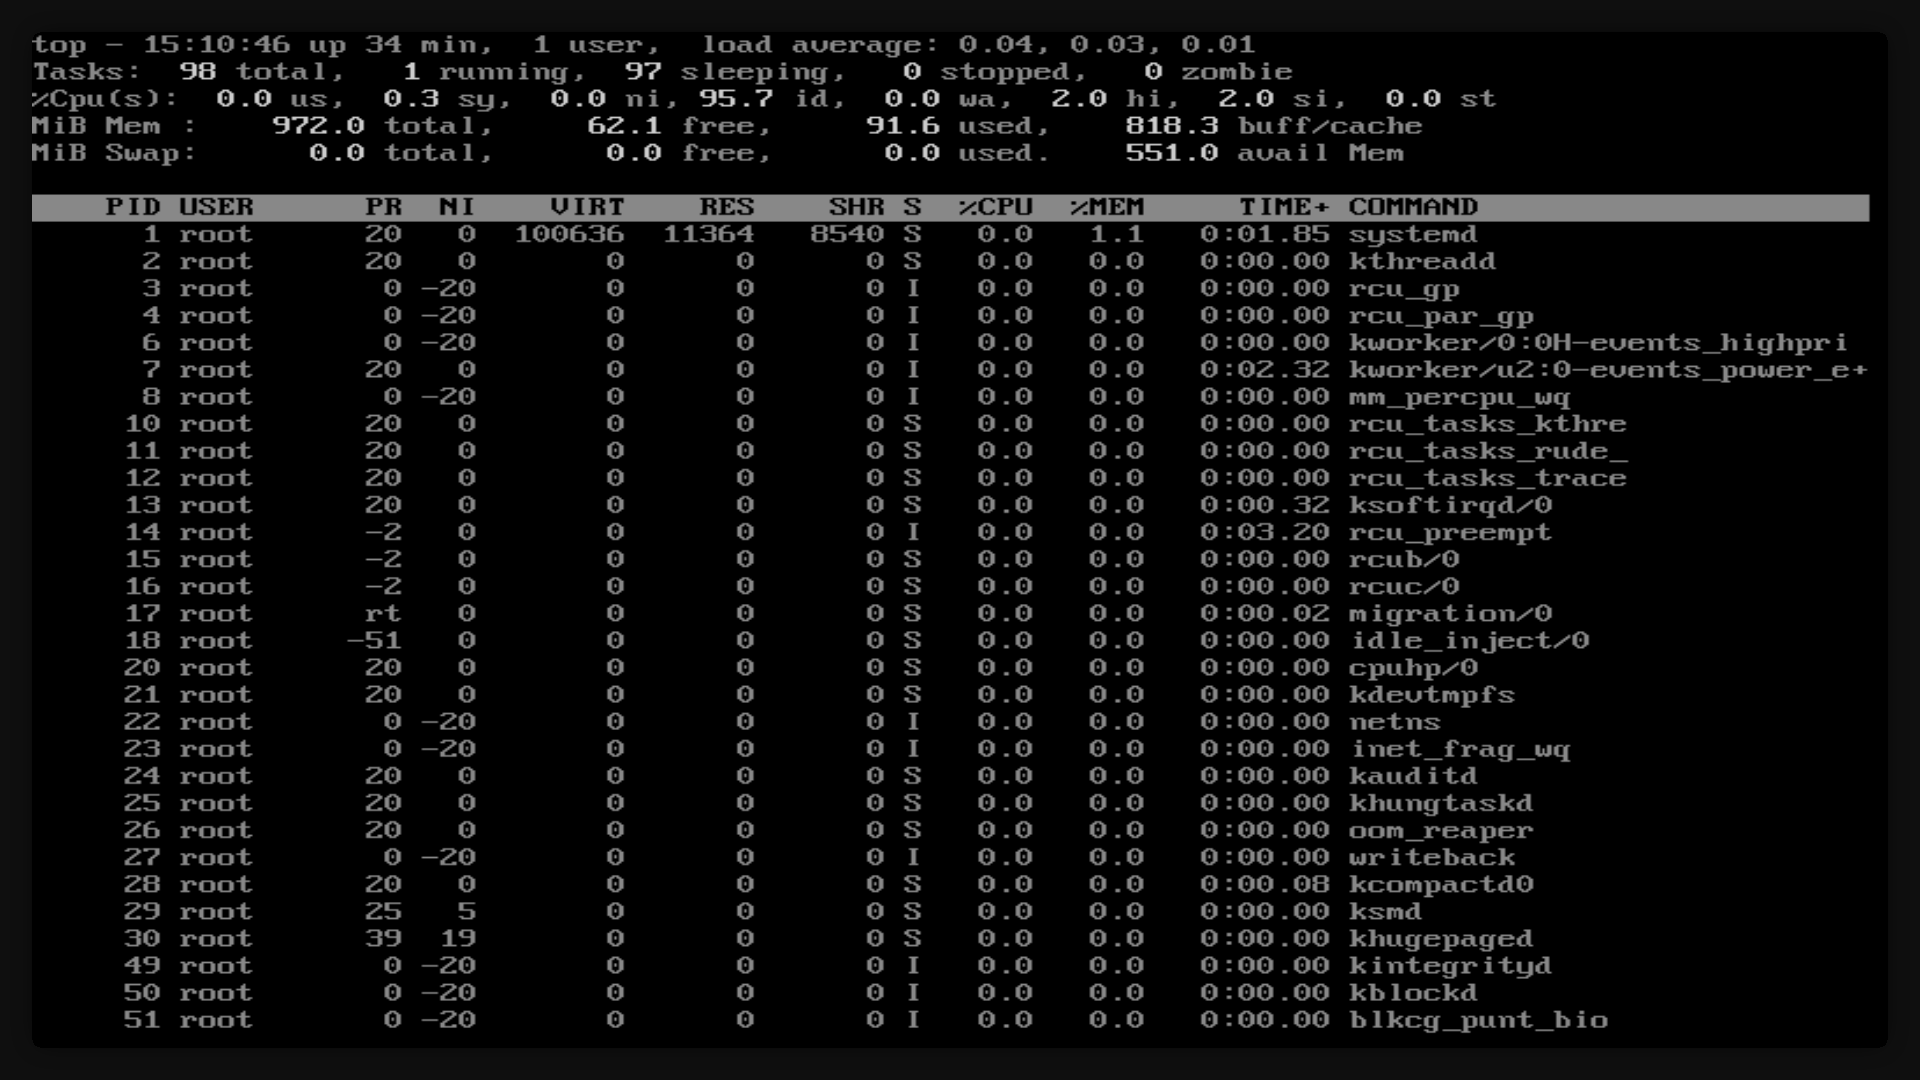
\includegraphics[width=\textwidth,clip=true]{img/3.png}
			\caption{Снова проверяем объем файла подкачки, который теперь равен 1024
			МиБ}
		\end{figure}

	\section{Создание пустого файла и монтирование его как файловую систему}
		\begin{figure}[H]
			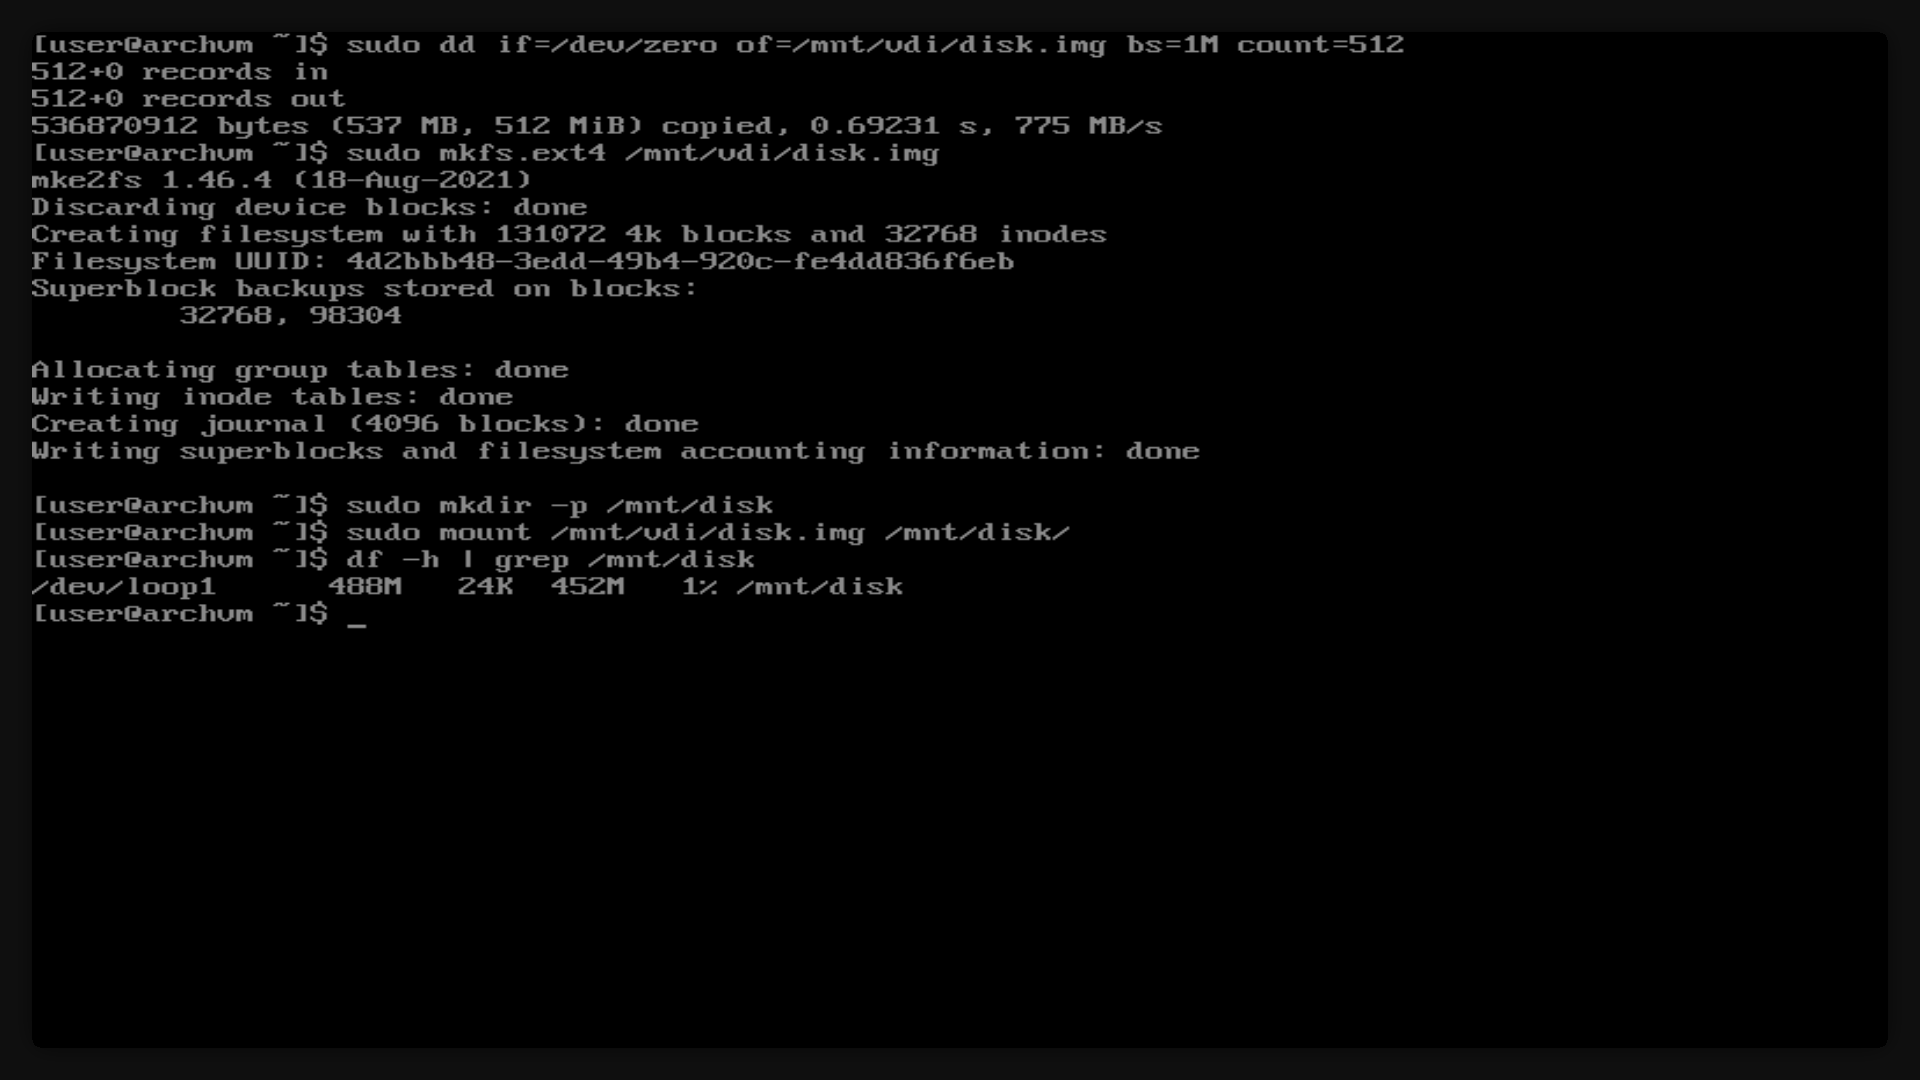
\includegraphics[width=\textwidth,clip=true]{img/4.png}
			\caption{Создаем пустой файл размером 512 МиБ, создаем на нем файловую
			систему ext4 и монтируем его в директорию /mnt/disk}
		\end{figure}
\end{document}
